% !TeX spellcheck = en_US
\documentclass[10pt,a4paper,titlepage]{article}
\usepackage[latin1]{inputenc}
\usepackage{amsmath}
\usepackage{amsfonts}
\usepackage{amssymb}
\usepackage{makeidx}
\usepackage{graphicx}
\usepackage[left=2.00cm, right=2.00cm, top=2.00cm, bottom=2.00cm]{geometry}
\usepackage{tikz}
\usepackage{tikz-uml}
\usetikzlibrary{patterns}%for tikz https://tex.stackexchange.com/questions/54464/hatch-a-rectangle-in-tikz
%sources
\usepackage[backend=bibtex]{biblatex}
\bibliography{Thesis}
%Makes index browsable in pdf viewers and shows index in sidebar
\usepackage[bookmarks]{hyperref}
\author{Mikail Gedik}
\title{Thesis Paper}
\begin{document}
	\pagenumbering{roman}
	\maketitle
	\tableofcontents
	\listoffigures
	\clearpage
	\pagenumbering{arabic}
	
	\section{Abstract}
	This paper tackles the calculation of a few selected fractals and shines light on the core aspects I have implemented and furthermore optimized to use all the resources provided by the computer. My journey begins at a single threaded Java program and ends in a multi threaded C application able to make use graphics cards. Additionally, I will make an easy-to use yet powerful UI, which will enable even tech-unfamiliar people to use my software.
	\section{What are Fractals}
	Fractals are complex geometric shapes with special properties. But in contrast to normal finite Euclidean shapes (such as the circle, sphere, cube etc.), fractals are infinite. The angles and the lines of a cube are indifferent from the magnification. Fractals have the property that no matter how much they are magnified or zoomed into, the edges are never smooth but rough. New levels of detail will appear. Surprisingly, some fractals can even contain themselves. This property (well seen in the Sierpinski triangle, figure \ref{fig:sierpinski_triangle}) is called self-similarity. Although the self-similarity in this example is perfect, many fractals contain non-perfect copies of themselves. This can often be observed in nature, for example tree branches or snowflakes (figure \ref{fig:snowflake}).\\
	There are different types of fractals: geometric, algebraic and naturally occurring. Geometric and algebraic fractals are created by repeating a process over and over again. The Sierpinski triangle repeatedly cuts out the center piece of each black triangle \ref{fig:sierpinski_triangle_build}. The algebraic ones iterate have to iterate over an equation to determine its shape.\\
	While they were first conceptualized by Felix Hausdorff in 1918, the term fractal (from Latin fragmented, broken) was only coined in 1975 by mathematician Benoit B. Mandelbrot. A factor in this long time span were the invention of computers, which made the exploration of fractals much easier due to their impressive computation power. Mandelbrot used fractals as a tool to examine the stock market, but were also found to be useful in various fields like physical chemistry, fluid mechanics and physiology. \cite{FractalFoundation}, \cite{FractalFoundation}, \cite{britannica}.
	\begin{figure}[h]
		\caption{Sierpi?ski triangle [\cite{Sierpinski}]}
		\label{fig:sierpinski_triangle}
		\centering
		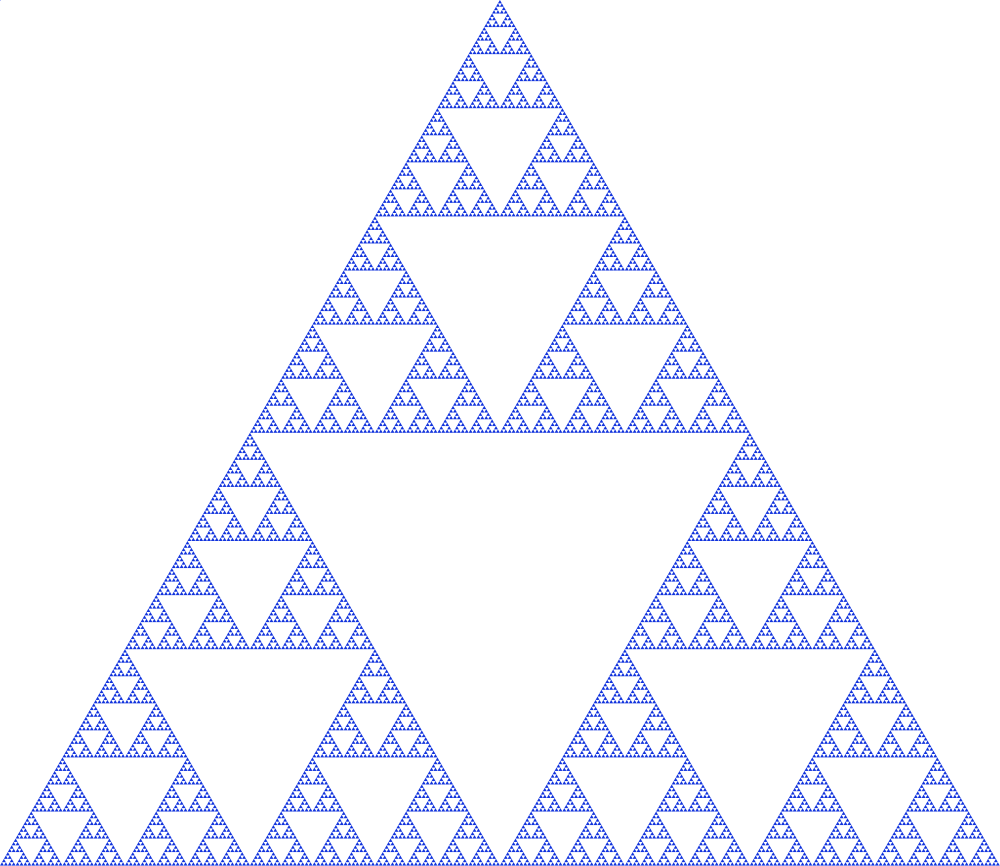
\includegraphics[width=0.5\textwidth]{"res/images/1000px-Sierpinski_triangle.svg.png"}
	\end{figure}
	\begin{figure}[h]
		\caption{Each branch of the snowflake creates new smaller branches \cite{wikipedia_snowflake}}
		\label{fig:snowflake}
		\centering
		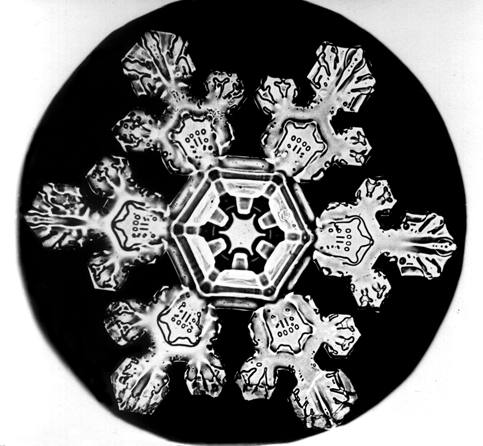
\includegraphics[width=0.5\textwidth]{"res/images/bentley_snowflake.jpg"}
	\end{figure}
	\begin{figure}[h]
		\caption{Creation of the Sierpinski triangle}
		\label{fig:sierpinski_triangle_build}
		\centering
		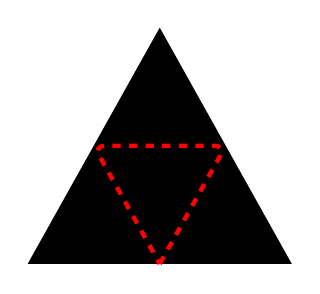
\begin{tikzpicture}[scale=3]
		\fill[black] (0,0) -- (1.118,0) -- (1.118/2, 1);
		
		\draw[rounded corners, dashed, red, ultra thick] (1.118/2, 0) -- (1.118/4*3,.5) -- (1.118/4, .5) -- (1.118/2, 0);
		\end{tikzpicture}
		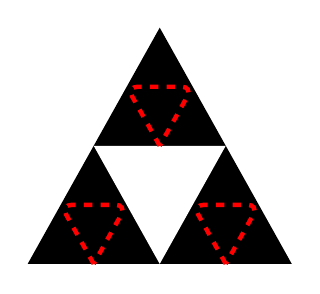
\begin{tikzpicture}[scale=3]
		\fill[black] (0,0) -- (1.118033989,0) -- (1.118033989/2, 1);
		\fill[white] (1.118/2, 0) -- (1.118/4*3,.5) -- (1.118/4, .5);
		
		\draw[rounded corners, dashed, red, ultra thick] (1.118/4*3, 0) -- (1.118/8*5,.25) -- (1.118/8*7, .25) -- (1.118/4*3, 0);
		\draw[rounded corners, dashed, red, ultra thick] (1.118/4, 0) -- (1.118/8,.25) -- (1.118/8*3, .25) -- (1.118/4, 0);
		\draw[rounded corners, dashed, red, ultra thick] (1.118/2, .5) -- (1.118/8*3,.75) -- (1.118/8*5, .75) -- (1.118/2, .5);
		\end{tikzpicture}
		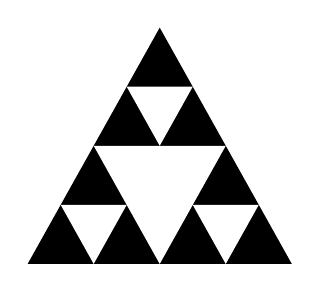
\begin{tikzpicture}[scale=3]
		\fill[black] (0,0) -- (1.118033989,0) -- (1.118033989/2, 1);
		
		\fill[white] (1.118/2, 0) -- (1.118/4*3,.5) -- (1.118/4, .5);
		
		\fill[white] (1.118/4*3, 0) -- (1.118/8*5,.25) -- (1.118/8*7, .25);
		\fill[white] (1.118/4, 0) -- (1.118/8,.25) -- (1.118/8*3, .25);
		\fill[white] (1.118/2, .5) -- (1.118/8*3,.75) -- (1.118/8*5, .75);
		\end{tikzpicture}
	\end{figure}
	
	%finite fractal contains infinity/self-similarity. occurs in nature. equally rough at all scales. not possible to understand with classical geometry\cite{FractalsForDummies}.\\
	%Never ending repeating branching pattern. (Infinitely complex). Made by repeating simple process often. Geometric fractals created by repeating simple process (sierpinski triangle). Algebraic fractals: repeat equation over and over \cite{FractalFoundation}:\\
	%complex geometric shapes. Concept by Felix Hausdorff 1918. Are distinct from classical/Euclidean geometry (square, circle, sphere etc.). spatially nonuniform phenomena in nature (coastlines, mountain ranges). Word fractal (Latin for "fragmented", "broken") by mathematician Benoit B. Mandelbrot. Fractals as tools for different fields (stock market). Self-similar objects have remain invariant under changes of scale: they have scaling symmetry. Fractal dimension vs. euclidean dimension, a noninteger. Fractals are used to simulate nature (e. g. tree branches)\cite{britannica}
	
	\section{The Mandelbrot Set}
	Although the most part of my thesis paper is dedicated to computer science the necessity arises to explain the most used fractal in my work. The Mandelbrot set was named after Benoit Mandelbrot, and is the first one to be called a fractal. In terms of properties, it is related to the Julia set, which is not a part of my work, albeit my program has the ability to display them. The Mandelbrot set is an algebraic fractal in the complex plane \(z = a + b i\). To find out which points are part of the set, we have to repeatedly apply the function \(z_{n+1} = z_{n}^2 + c\) to every point \(z\) in the plane. If the point diverges (or is known to diverge) as \(n\) approaches infinity, it is said to be outside the set. The most interesting points lie at the boundary of the set, as the edge is the most interesting part of any fractal.
	
	%named after benoit mandelbrot. related to julia set. choose complex number \(c\) and \(z_0\) and repeatedly put into equation \(z_n = z_{n+1} + c\). If \(z_n\) diverges, point not in fractal. Interesting points near boundary \cite{freeuk}
	\section{The Program}
	This section represents the core of my paper. The capabilities, structure and implementation are discussed in depth
	\subsection{Program Functionalities}
	\subsection{Structure}
	\subsubsection{Core}
	\subsubsection{GUI}
	\subsubsection{Connector}
	\subsection{Implementation}
	\subsubsection{Data Management}
	
	\subsubsection{GUI}
	\section{Workflow and Major Version History}
\end{document}